\section{Results}
\label{sec:results}
% =====================================================================

\subsection{DESI-like mocks: ASTRA split, density split and the 2PCF}

Table~\ref{tab:sigma} gives the baseline errors and Figure~\ref{fig:ratios} the ratios between the two methods for several data vectors. Three results stand out. Both environment statistics improve on the 2PCF on every parameter, by factors 1.6--3.1. They carry comparable information: density split is slightly ahead on most parameters, by 6--17\%, ASTRA on $\omega_{\rm cdm}$, but all these differences are within 1.7 times the uncertainty from the emulator training (last row of Table~\ref{tab:sigma}). And they are complementary: their combination improves on the better of the two by 23\% ($\sigma_8$) to a factor 2.4 ($\omega_b$). The errors on $w_0$ and $w_a$ ($\simeq0.8$ and 2.7) are larger than the range spanned by the AbacusSummit suite: one $(500\Mpch)^3$ volume does not constrain the dark-energy parameters, and only the relative information content is meaningful for them. Freeing $w_0$ and $w_a$ changes the other ASTRA errors by at most $+42\%$ (on $\omega_{\rm cdm}$; $+16\%$ on $n_s$, $\le3\%$ on $\omega_b$ and $\sigma_8$) and the DS/ASTRA ratios by less than their uncertainty. The other data vectors (auto-correlations, galaxy quartiles, single environments) give ratios between 0.48 and 1.40, detailed below.

\begin{table}[!htbp]
\centering\small
\begin{adjustbox}{max width=\linewidth}
\begin{tabular}{lcccccc}
\toprule
data vector & $\omega_b$ & $\omega_{\rm cdm}$ & $n_s$ & $\sigma_8$ & $w_0$ & $w_a$ \\
\midrule
2PCF & 0.033 & 0.057 & 0.40 & 0.58 & 2.1 & 6.7 \\
ASTRA & 0.012 & 0.032 & 0.22 & 0.23 & 0.80 & 2.7 \\
DS & 0.011 & 0.035 & 0.18 & 0.19 & 0.75 & 2.5 \\
ASTRA + DS & 0.0046 & 0.022 & 0.13 & 0.15 & 0.53 & 1.5 \\
2PCF + ASTRA + DS & 0.0039 & 0.019 & 0.12 & 0.13 & 0.50 & 1.3 \\
\midrule
$\sigma_{\rm DS}/\sigma_{\rm ASTRA}$ & 0.90(11) & 1.10(16) & 0.84(15) & 0.83(10) & 0.94(11) & 0.92(9) \\
\bottomrule
\end{tabular}
\end{adjustbox}
\caption{Baseline marginalised $1\sigma$ errors (random-quartile Q1+Q4 cross-correlations, HOD marginalised) for one $(500\Mpch)^3$ volume, and ratio of the density-split and ASTRA errors (above 1: ASTRA more constraining; in parentheses, uncertainty from the emulator training on the last digits). The errors are comparable to the prior widths: they compare information content and are not realistic constraints.}
\label{tab:sigma}
\end{table}

Figure~\ref{fig:triangle} shows the corresponding contours. Reading such a figure: each panel shows the region of two parameters allowed at 68\% and 95\% confidence, the others being marginalised; a smaller ellipse means a tighter constraint, and an elongated, tilted ellipse a degeneracy (the two parameters can compensate each other). The environment statistics shrink the contours of the 2PCF in every direction; the strong anti-correlation between $w_0$ and $w_a$ remains for all statistics.

\paragraph{What each environment contributes.} Table~\ref{tab:breakdown} gives the gain over the 2PCF of each quartile and of their combinations, and Figures~\ref{fig:q_astra}--\ref{fig:c_ds} show the corresponding contours in the layout of the density-split analyses. A single quartile is about as constraining as the 2PCF (gain 0.5--2.2), with one exception: the ASTRA Q3, 2 to 10 times less constraining than the 2PCF. Its information is however of a different nature: the 2PCF averages the clustering over all environments, whereas a quartile measures it around one range of densities, e.g.\ the galaxy profile around voids for Q1. Because the environments respond differently to the parameters (opposite signs for Q1 and Q4, different scale dependences; Figures~\ref{fig:der_astra}, \ref{fig:der_ds}), combining them is what gains: Q1 and Q4 together improve on the 2PCF by 1.6--3.1, all four quartiles by 2.2--6.6, i.e.\ 1.6--3.6 times better than the best single quartile. The comparison of the two methods environment by environment is informative. In the voids (Q1) they are equivalent. In the dense regions (Q4), ASTRA is more constraining on $n_s$ (1.5 vs 0.9) and $\sigma_8$ (2.0 vs 1.7), density split on $\omega_b$ and $\omega_{\rm cdm}$. With all four quartiles density split is ahead, mostly because of the weak ASTRA Q3. We have not identified the cause of this weakness; a plausible one is that $r$ takes few discrete values, so that the intermediate quartiles are largely set by the random tie-breaking between equal values.

\begin{table*}[!tp]
\centering\small
\begin{adjustbox}{max width=\textwidth}
\begin{tabular}{lcccccc}
\toprule
cross-correlations & $\omega_b$ & $\omega_{\rm cdm}$ & $n_s$ & $\sigma_8$ & $w_0$ & $w_a$ \\
\midrule
Q1 & 0.9 / 0.9 & 0.9 / 0.9 & 1.3 / 1.3 & 1.5 / 1.4 & 1.6 / 1.7 & 1.6 / 1.7 \\
Q2 & 1.4 / 1.0 & 0.6 / 0.5 & 0.5 / 0.7 & 1.0 / 1.5 & 1.7 / 2.2 & 1.6 / 2.0 \\
Q3 & 0.5 / 1.7 & 0.1 / 0.7 & 0.2 / 0.9 & 0.1 / 0.8 & 0.3 / 1.1 & 0.2 / 0.8 \\
Q4 & 1.3 / 1.6 & 1.1 / 1.3 & 1.5 / 0.9 & 2.0 / 1.7 & 1.6 / 1.6 & 1.5 / 1.8 \\
Q1+Q4 & 2.8 / 3.0 & 1.8 / 1.6 & 1.9 / 2.2 & 2.5 / 3.1 & 2.6 / 2.8 & 2.4 / 2.7 \\
Q1--Q4 & 5.2 / 4.6 & 2.2 / 2.6 & 2.4 / 3.1 & 3.5 / 3.6 & 4.6 / 6.6 & 3.8 / 4.7 \\
Q1 + auto & 1.8 / 3.6 & 1.4 / 2.0 & 1.7 / 1.9 & 2.3 / 2.1 & 2.9 / 2.7 & 2.7 / 2.8 \\
Q4 + auto & 3.9 / 5.7 & 1.6 / 2.1 & 2.2 / 2.3 & 3.8 / 2.7 & 4.0 / 3.8 & 2.9 / 3.7 \\
Q1+Q4 + auto & 6.4 / 8.5 & 2.3 / 3.3 & 2.7 / 3.7 & 4.7 / 4.2 & 5.5 / 5.3 & 4.4 / 5.3 \\
\bottomrule
\end{tabular}
\end{adjustbox}
\caption{Gain over the 2PCF, $\sigma_{\rm 2PCF}/\sigma$, for single quartiles and combinations, ASTRA split / density split (baseline: official covariance and fiducial point, six parameters, HOD marginalised, one $(500\Mpch)^3$ volume). Above 1: more constraining than the 2PCF. The uncertainty due to the emulator training is $\sim10\%$.}
\label{tab:breakdown}
\end{table*}

\paragraph{Auto-correlations.} Adding the quartile auto-correlations tightens the constraints of both methods by factors 1.3--2.8 depending on the parameter (Figure~\ref{fig:autocross}). The two methods remain comparable (ratios 0.69--1.13): density split is ahead on $\omega_b$, $\omega_{\rm cdm}$ and $n_s$ (by 24--31\%), mostly through its void auto-correlation, and ASTRA on $\sigma_8$ (by 13\%), through its dense-region auto-correlation (Table~\ref{tab:breakdown}: gain 3.8 vs 2.7 for Q4 with its auto-correlation).

\paragraph{Scale cuts.} Figure~\ref{fig:smin} shows the errors as a function of the minimum scale. All statistics lose information as small scales are removed. The environment statistics stay 0.15--0.51 dex (factors 1.4--3.2) below the 2PCF up to $s_{\min}=70\Mpch$ (beyond, the 2PCF has fewer bins than parameters). ASTRA and density split stay within 0.08 dex (20\%) of each other at all scale cuts, except on $\omega_b$ (0.15 dex), their ranking changing with $s_{\min}$, and their combination remains 0.09--0.37 dex below the better of the two.

\paragraph{Fiducial point.} Evaluated at four different HODs, the ratio $\sigma_{\rm DS}/\sigma_{\rm ASTRA}$ stays between 0.77 and 1.14 for all six parameters (Table~\ref{tab:covbox}): the comparison depends on the fiducial galaxy population at the $\pm15\%$ level, the same order as the differences between the methods.

\begin{table}[!htbp]
\centering\small
\begin{adjustbox}{max width=\linewidth}
\begin{tabular}{lcccccc}
\toprule
fiducial HOD & $\omega_b$ & $\omega_{\rm cdm}$ & $n_s$ & $\sigma_8$ & $w_0$ & $w_a$ \\
\midrule
official & 0.90(11) & 1.10(16) & 0.84(15) & 0.83(10) & 0.94(11) & 0.92(9) \\
\texttt{hod239} & 0.83(9) & 0.92(7) & 1.04(12) & 0.93(8) & 0.88(6) & 0.84(8) \\
\texttt{hod212} & 0.77(7) & 0.94(9) & 0.94(13) & 0.84(8) & 0.85(8) & 0.89(10) \\
\texttt{hod795} & 0.79(8) & 0.98(10) & 1.06(16) & 1.14(10) & 0.89(12) & 0.92(13) \\
\bottomrule
\end{tabular}
\end{adjustbox}
\caption{$\sigma_{\rm DS}/\sigma_{\rm ASTRA}$ (above 1: ASTRA ahead) for the random-quartile cross-correlations with the official covariance at four fiducial HODs; in parentheses, the uncertainty from the emulator training.}
\label{tab:covbox}
\end{table}

\begin{figure}[!htbp]
\centering
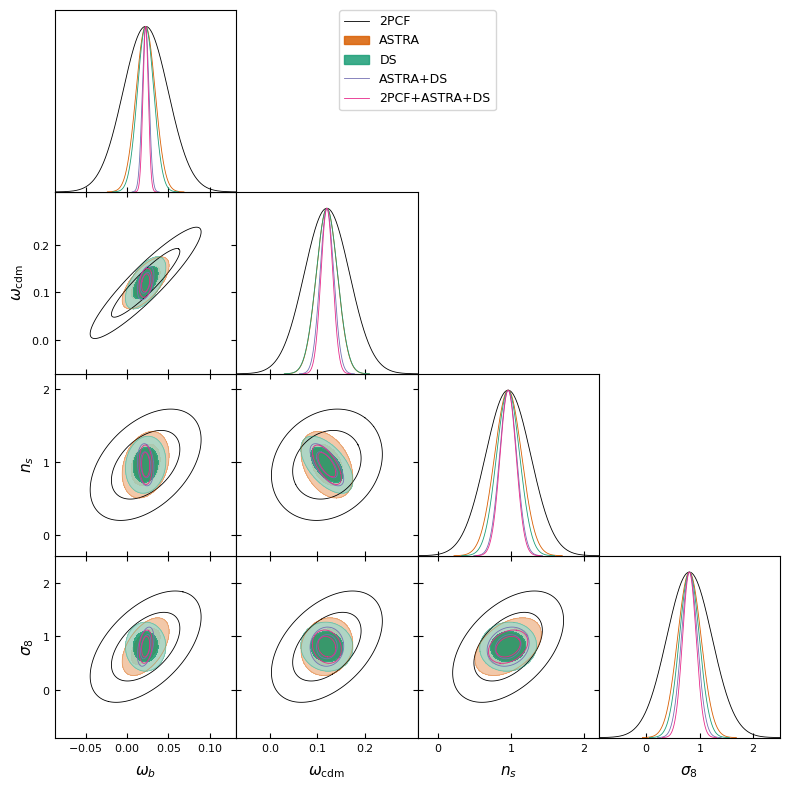
\includegraphics[width=\linewidth]{v2_triangle.png}
\caption{Baseline Fisher contours (68\% and 95\%) for the 2PCF, ASTRA split, density split and their combinations, one $(500\Mpch)^3$ volume, HOD marginalised.}
\label{fig:triangle}
\end{figure}

\begin{figure}[!htbp]
\centering
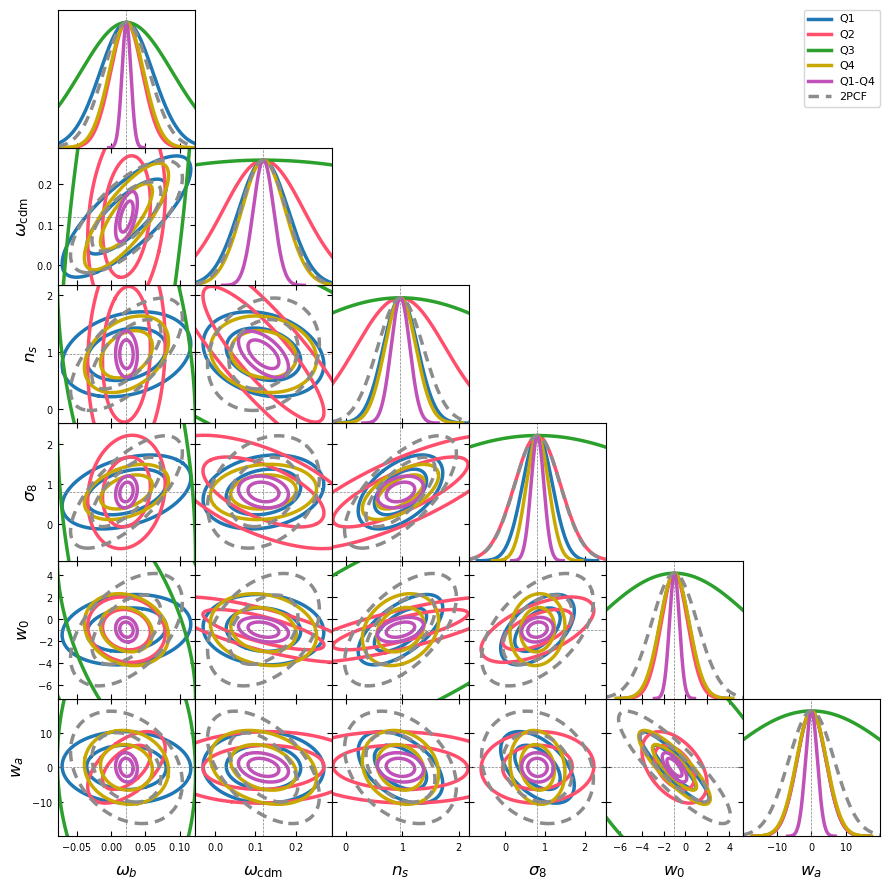
\includegraphics[width=\linewidth]{v1style_quartiles_astra.png}
\caption{Constraints (68\% and 95\%) from individual and combined ASTRA-split quartiles (cross-correlations) and from the 2PCF (dashed), baseline, HOD marginalised. Axes span $\pm3\sigma$ of the 2PCF.}
\label{fig:q_astra}
\end{figure}

\begin{figure}[!htbp]
\centering
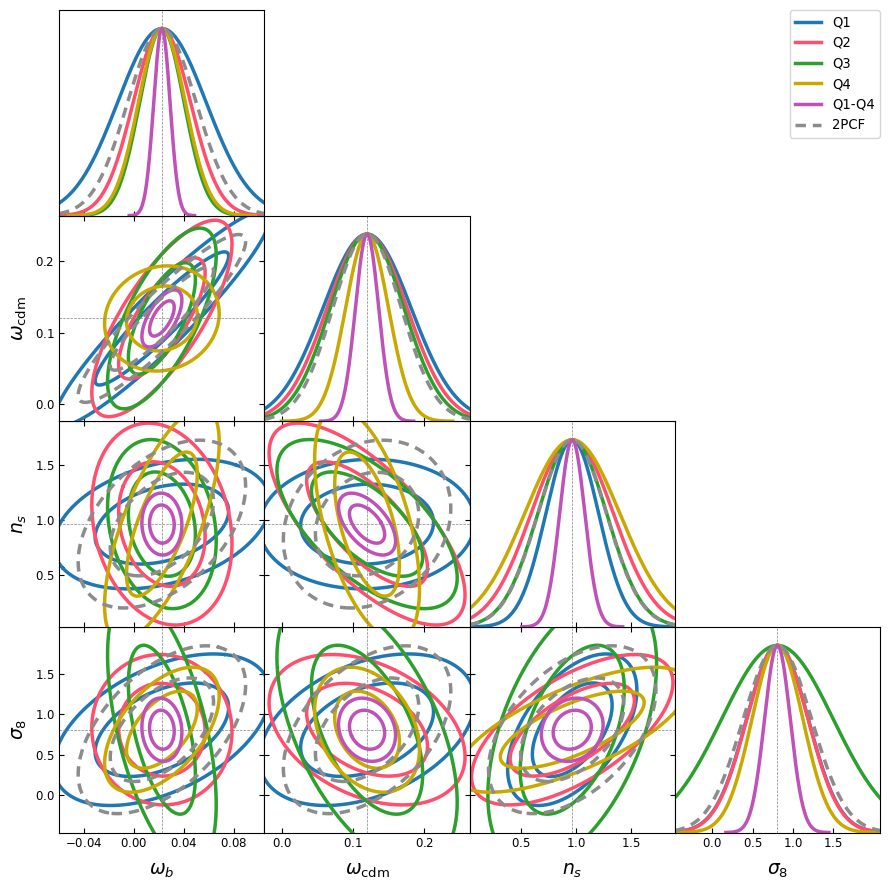
\includegraphics[width=\linewidth]{v1style_quartiles_ds.png}
\caption{Same as Figure~\ref{fig:q_astra} for density split.}
\label{fig:q_ds}
\end{figure}

\begin{figure}[!htbp]
\centering
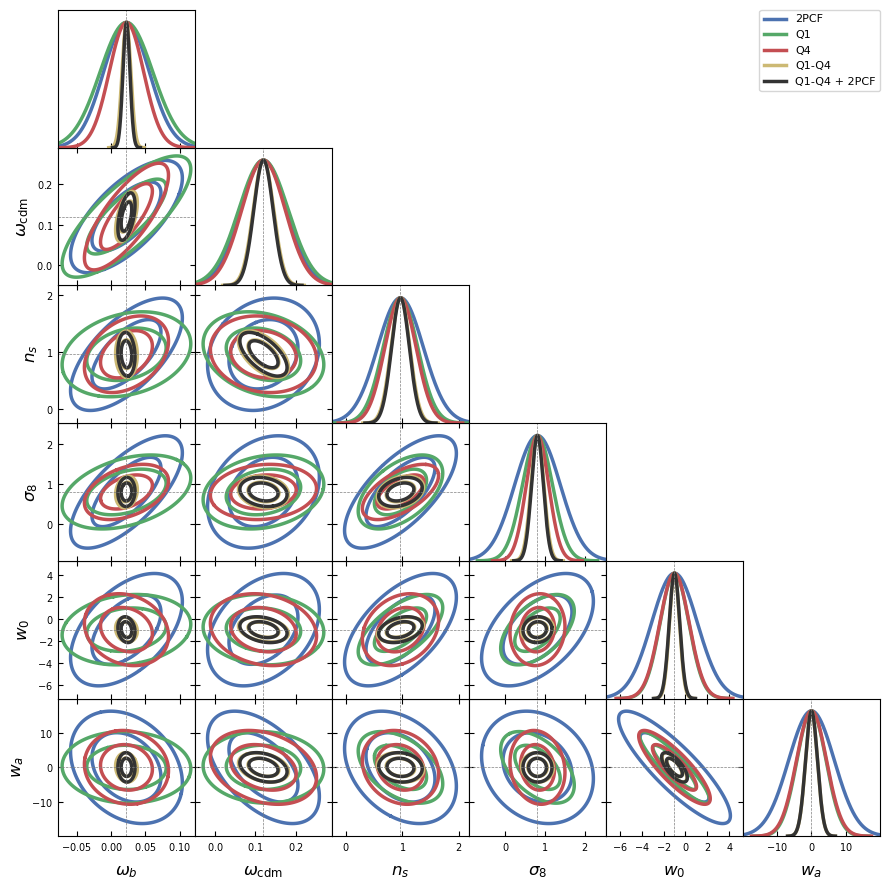
\includegraphics[width=\linewidth]{v1style_constraints_astra.png}
\caption{ASTRA split: constraints from the 2PCF, the Q1 and Q4 cross-correlations, all quartiles, and all quartiles with the 2PCF (baseline).}
\label{fig:c_astra}
\end{figure}

\begin{figure}[!htbp]
\centering
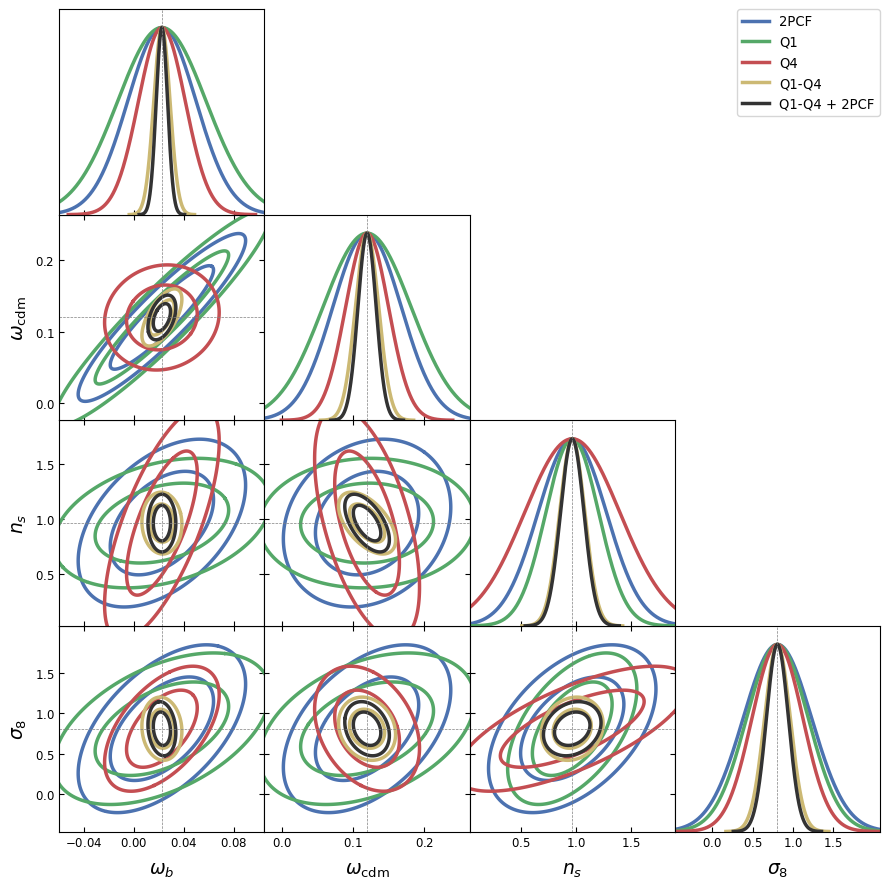
\includegraphics[width=\linewidth]{v1style_constraints_ds.png}
\caption{Same as Figure~\ref{fig:c_astra} for density split.}
\label{fig:c_ds}
\end{figure}

\begin{figure*}[!tp]
\centering
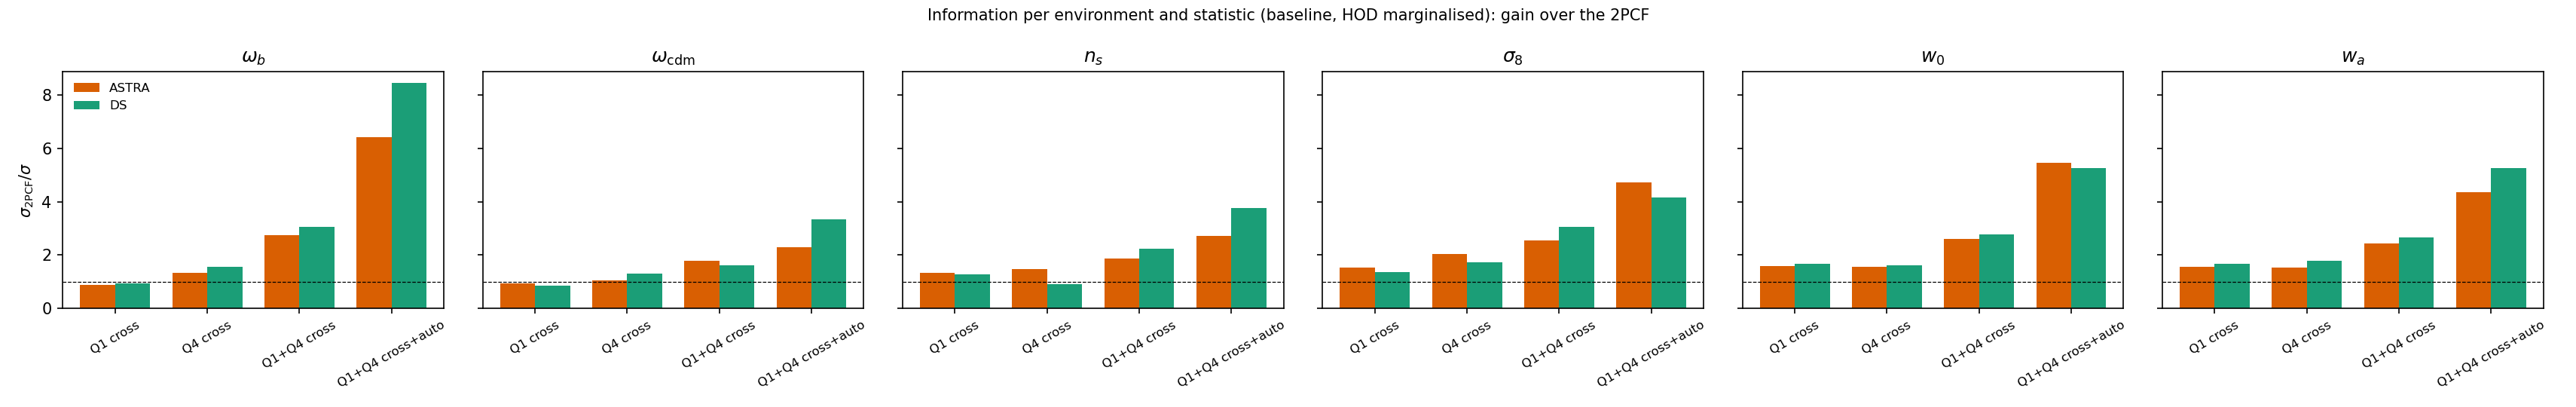
\includegraphics[width=\textwidth]{v2_quartiles.png}
\caption{Gain over the 2PCF, $\sigma_{\rm 2PCF}/\sigma$, for the Q1 and Q4 cross-correlations alone, together, and with the quartile auto-correlations, for ASTRA split (orange) and density split (green) (baseline, HOD marginalised).}
\label{fig:quartiles}
\end{figure*}

\begin{figure}[!htbp]
\centering
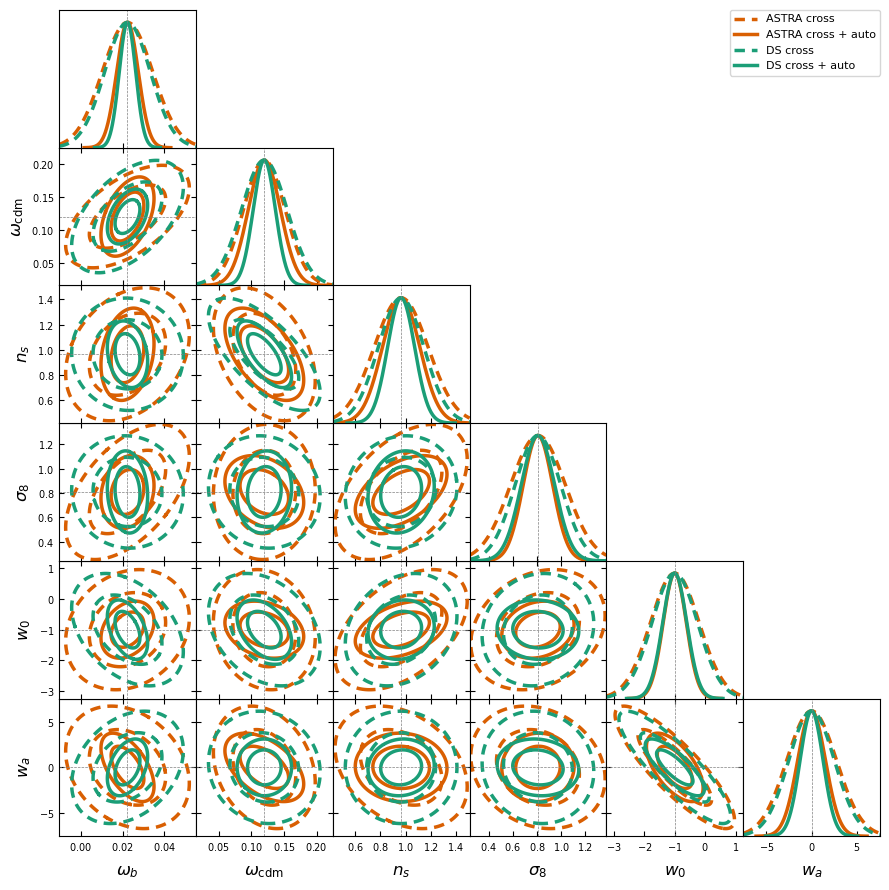
\includegraphics[width=\linewidth]{v1style_autocross.png}
\caption{Q1+Q4 cross-correlations only (dashed) and with the quartile auto-correlations (solid), for ASTRA split (orange) and density split (green), baseline.}
\label{fig:autocross}
\end{figure}

\begin{figure}[!htbp]
\centering
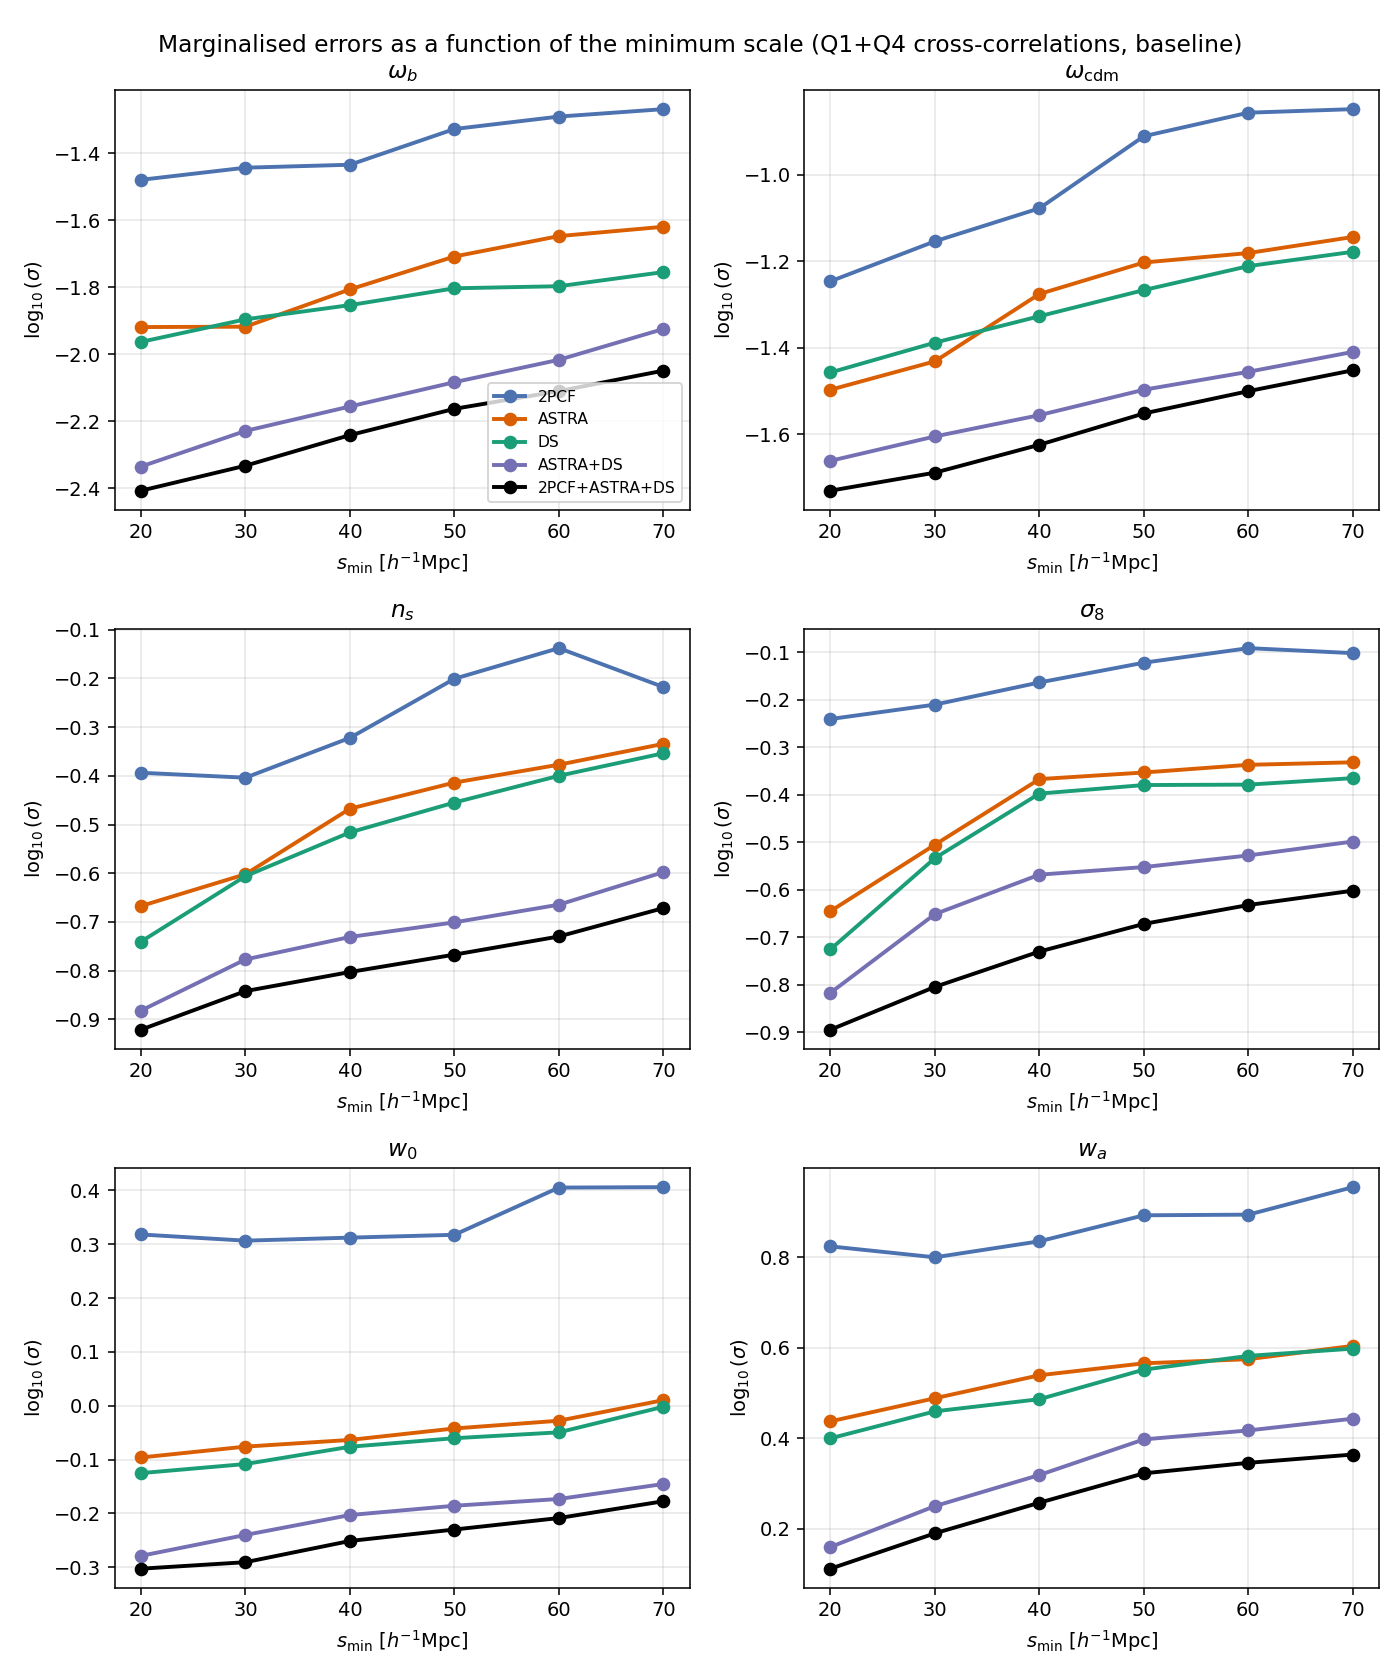
\includegraphics[width=\linewidth]{v1style_smin.png}
\caption{Marginalised errors as a function of the minimum scale $s_{\min}$ (Q1+Q4 cross-correlations, baseline).}
\label{fig:smin}
\end{figure}

\begin{figure*}[!tp]
\centering
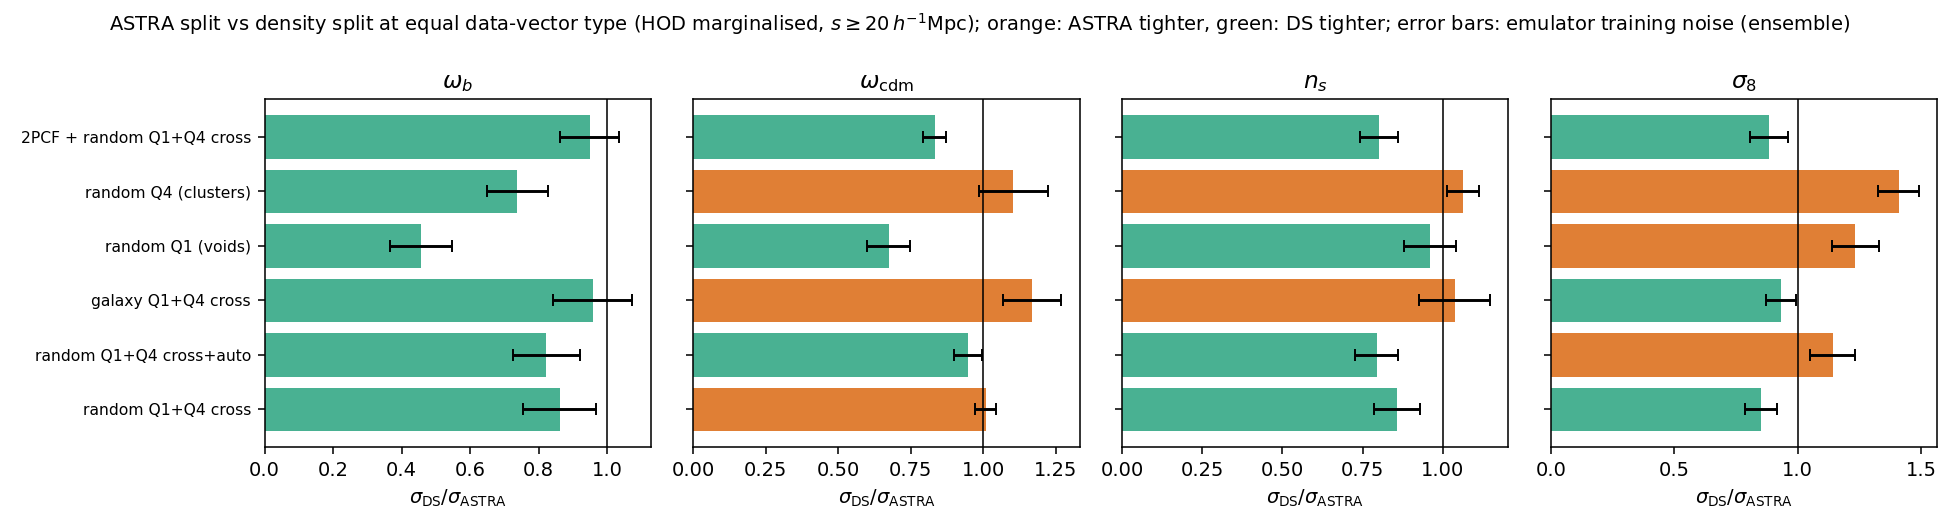
\includegraphics[width=\textwidth]{v2_compare_ratios.png}
\caption{Baseline: $\sigma_{\rm DS}/\sigma_{\rm ASTRA}$ for several data-vector types (above 1: ASTRA split more constraining). Error bars: uncertainty from the emulator training.}
\label{fig:ratios}
\end{figure*}

\begin{figure*}[!tp]
\centering
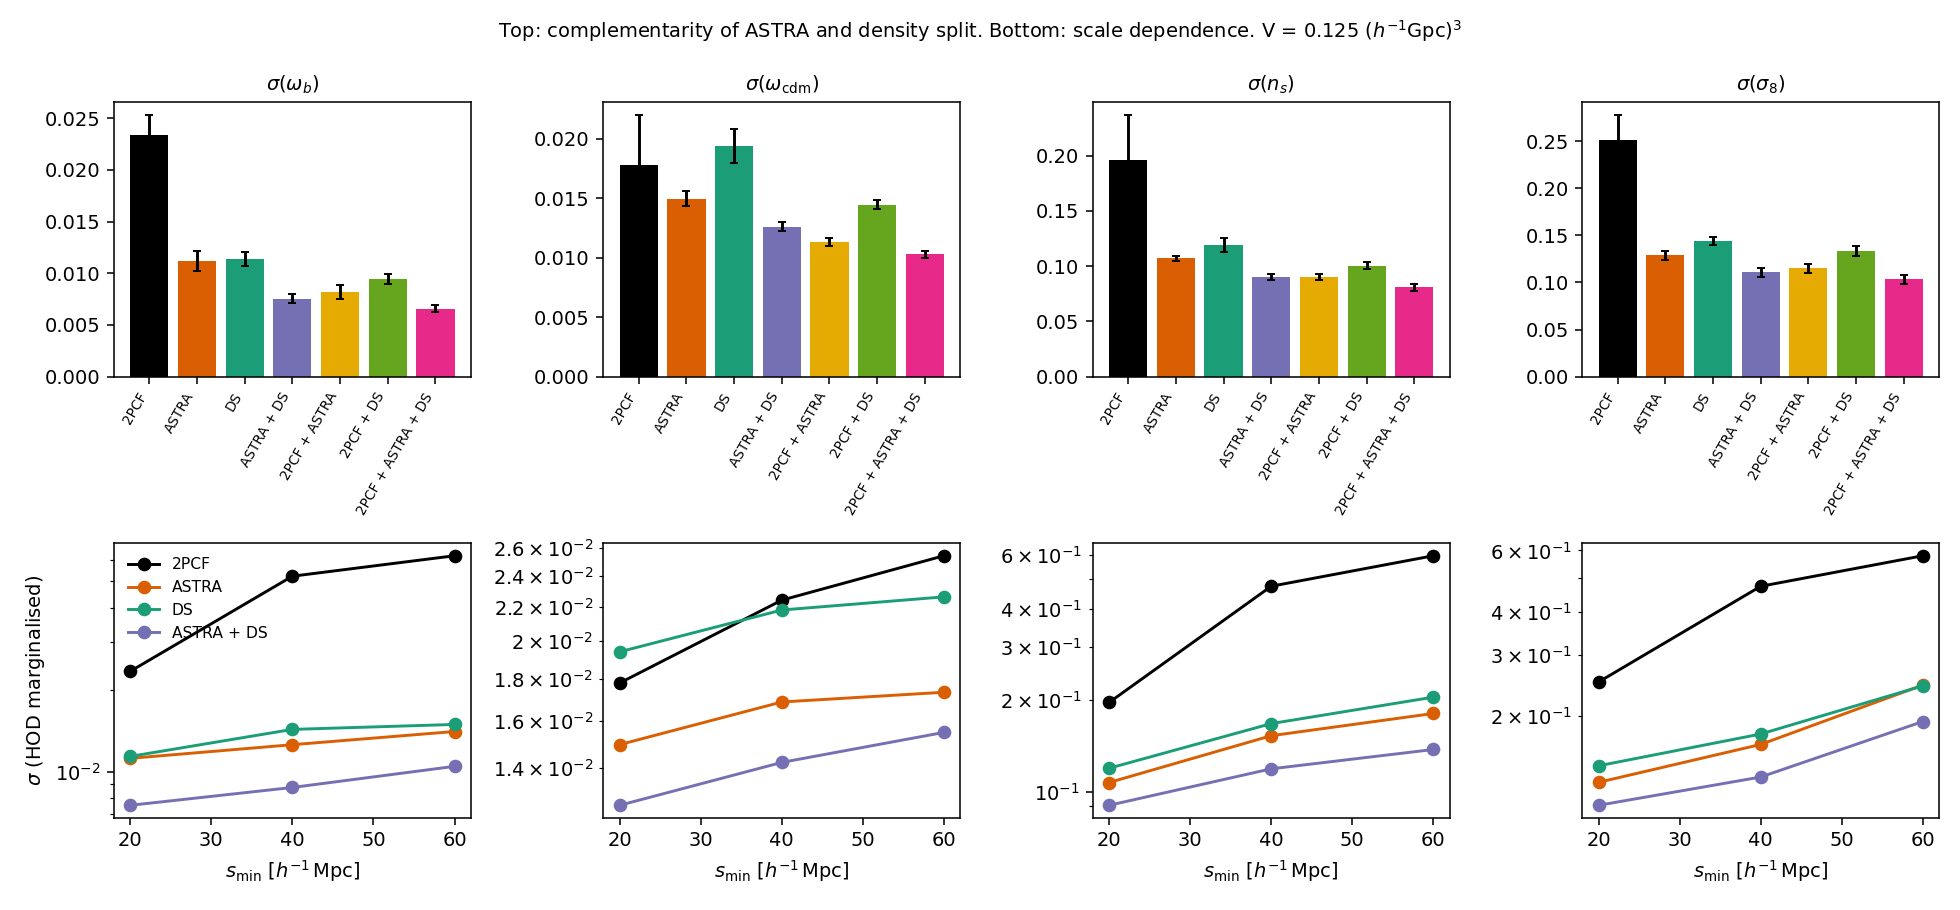
\includegraphics[width=\textwidth]{v2_compare_combined.png}
\caption{Baseline. Top: marginalised errors of the 2PCF, ASTRA split, density split and their combinations. Bottom: dependence on the minimum scale.}
\label{fig:combined}
\end{figure*}

\subsection{Quijote halos}
\label{sec:quijote}

\paragraph{Covariance.} We use 4000 fiducial realisations, enough for the covariance: for the parameter sets retained below, the marginalised errors change by less than 4\% between 1000 and 4000 realisations and by less than 3\% between 2000 and 4000, at fixed derivatives.

\paragraph{Pairing.} The $\pm$ realisations of a given index share their initial conditions: the scatter of the differences between realisations of the same index is 2.5--3.8 times smaller than between different indices, for the 2PCF as for the quartile statistics.

\paragraph{Noise of the derivatives.} Even paired, the derivatives remain noisy. Quijote is designed for statistics of the matter and halo fields (power spectrum, bispectrum, \dots). Our observables add two sources of noise that the pairing cannot cancel:
\begin{enumerate}
\item \emph{Sparse tracers.} With $\simeq50\,000$ host halos per $(h^{-1}{\rm Gpc})^3$, each quartile contains only $\simeq12\,000$ halos (or random points), and the shot noise of the quartile statistics is large.
\item \emph{Discrete classification.} A small change of cosmology moves halos and random points from one quartile to another. This re-classification is only partly common to the $+$ and $-$ simulations, even with identical initial conditions, and adds a noise that does not cancel in the difference.
\end{enumerate}
This noise matters most in the six-parameter Fisher matrix. $\Omega_b$, $h$ and $n_s$ (and $M_\nu$) are strongly degenerate in the clustering of halos: their weakest combination is constrained by a very small amount of information, of the same order as the noise left in the average of 500 derivative pairs, so that along this direction the derivatives are dominated by noise. The standard Fisher estimator is then biased high, and subtracting the expected noise term makes the six-parameter matrices non positive definite (Appendix~\ref{app:maths}).

\paragraph{Estimator and reliability criterion.} We therefore use the approach of \cite{CoultonWandelt2023}: the standard estimator is biased high by the derivative noise, a compressed estimator (half of the simulations define the compression, the other half measure its information) is biased low; the two bracket the true Fisher information, and their geometric mean is nearly unbiased. Where they agree, the forecast does not depend on the derivative noise: we call a forecast \emph{reliable} when the compressed and standard errors differ by less than a factor 1.5 for both statistics compared.

\paragraph{Choice of the parameters and of the compression.} The derivative noise grows with the length of the data vector and is concentrated in the degenerate directions of parameter space. We therefore computed the forecasts for six parameter subsets, from $(\Omega_m,\sigma_8)$ to all six parameters, and for three \emph{compressions} of the data vector, i.e.\ three ways of summarising the same measurements with fewer numbers: $10\Mpch$ bins with $\ell=0,2$ (26 numbers per statistic), $20\Mpch$ bins with $\ell=0,2$ (12), and $20\Mpch$ bins with the monopole only (6). A shorter data vector carries a little less information but much less derivative noise; if a conclusion is the same for the three compressions, it does not depend on this trade-off. The result is clear-cut (Figure~\ref{fig:qsubsets}). For $(\Omega_m,\sigma_8)$ the two estimators agree within 5\% for every data vector and compression. For $(\Omega_m,n_s,\sigma_8)$ they agree within a factor 1.5 in most cases (median ratio 1.34), except for the random-quartile vectors with the finest binning. As soon as $\Omega_b$, $h$ or $M_\nu$ are varied, they differ by a median factor 4--6, and up to more than 50: these forecasts are dominated by the noise, and the ranking of the methods changes from one compression to the next. These parameters cannot be constrained with these observables and 500 derivative pairs. Fixing $\Omega_b$ and $h$, as many density-split forecasts do, is justified by external constraints (BBN, CMB); $M_\nu$ would require denser tracers or many more derivative simulations.

\paragraph{Results.} The reliable forecasts are given in Table~\ref{tab:quijote}. For the random-quartile cross-correlations they agree with the DESI-like analysis: density split is as constraining as ASTRA split or more ($\sigma_{\rm DS}/\sigma_{\rm ASTRA}=0.57$--$1.14$). With the quartile auto-correlations, or with the halo quartiles, ASTRA split is more constraining on $\sigma_8$, by a factor 1.5--2.1; on $\Omega_m$ and $n_s$ the two methods are within a factor 1.4 of each other, in either direction depending on the parameter set. As in the DESI-like analysis, the advantage of ASTRA on $\sigma_8$ comes from the clustering of its environments with themselves and from the environments of the tracers, not from the tracer profiles around random environments.

\begin{table}[!htbp]
\centering\small
\begin{adjustbox}{max width=\linewidth}
\begin{tabular}{llccc}
\toprule
quartiles & parameters & $\Omega_m$ & $n_s$ & $\sigma_8$ \\
\midrule
random, cross & $\Omega_m,\sigma_8$ & 0.86--1.04 & -- & 0.65--0.81 \\
random, cross & $\Omega_m,n_s,\sigma_8$ & 0.57--0.64 & 0.68--0.74 & 1.04--1.14 \\
random, + auto & $\Omega_m,\sigma_8$ & 1.19--1.40 & -- & 1.54--2.11 \\
random, + auto & $\Omega_m,n_s,\sigma_8$ & 0.74--0.81 & 0.85--0.92 & 1.72--1.78 \\
halo, cross & $\Omega_m,\sigma_8$ & 1.18--1.21 & -- & 1.91--2.04 \\
halo, cross & $\Omega_m,n_s,\sigma_8$ & 1.16--1.20 & 1.17--1.23 & 1.54--1.70 \\
\bottomrule
\end{tabular}
\end{adjustbox}
\caption{Quijote, reliable forecasts: $\sigma_{\rm DS}/\sigma_{\rm ASTRA}$, range over the reliable compressions of the data vector (above 1: ASTRA ahead).}
\label{tab:quijote}
\end{table}

\begin{figure*}[!tp]
\centering
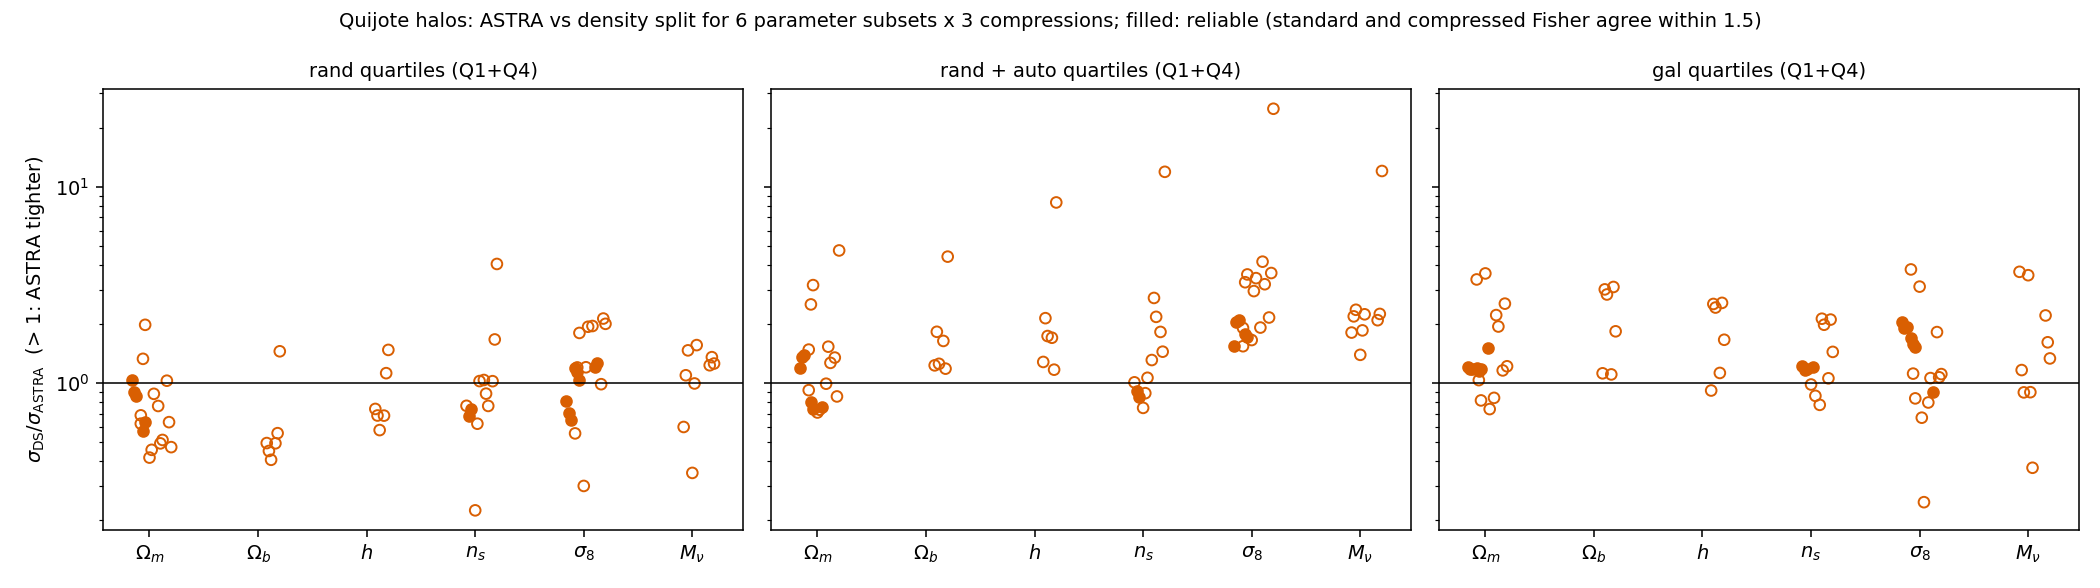
\includegraphics[width=\textwidth]{v2_quijote_subsets.png}
\caption{Quijote halos: $\sigma_{\rm DS}/\sigma_{\rm ASTRA}$ (above 1: ASTRA more constraining) for six parameter subsets and three compressions, for the random-quartile cross-correlations (left), with their auto-correlations (centre), and the halo quartiles (right). Filled: reliable forecasts (standard and compressed Fisher estimators within a factor 1.5); open: dominated by the noise of the derivatives.}
\label{fig:qsubsets}
\end{figure*}

\subsection{ASTRA cosmic-web classes (Quijote)}
\label{sec:classes}

To test whether the original ASTRA classes carry more information than quartiles, we measured them on Quijote, where the derivatives are clean: 4000 fiducial realisations for the covariance and the 500 pairs of $\Omega_m$, $n_s$ and $\sigma_8$, with the same halos, random points and estimators as the quartile analysis, and compared them with the quartiles of ASTRA and density split measured on the same realisations, for the three compressions defined in Section~\ref{sec:quijote}. Because the void and knot classes are nearly empty for random points, the class data vectors use the sheets and filaments (adding the voids changes the errors by less than 2\%).

\paragraph{Class fractions.} The fractions of points in each class are themselves sensitive to cosmology (Figure~\ref{fig:classes_resp}): a variation of $\Omega_m$, $n_s$ or $\sigma_8$ shifts the sheet and filament fractions of the random points by 0.3--1 times their scatter between realisations, in opposite directions. Unlike quartiles, which have fixed fractions by construction, fixed thresholds let the volume of each environment respond to cosmology.

\paragraph{Information.} Table~\ref{tab:classes} and Figure~\ref{fig:classes_fisher} give the comparison. With cross-correlations only, the classes are within 30\% of the ASTRA quartiles and 13--40\% less constraining than density split on $\sigma_8$: the classes bring nothing by their profiles alone. With the auto-correlations, they are the most constraining statistic for every compression. For $(\Omega_m,\sigma_8)$, all forecasts are reliable, and $\sigma(\sigma_8)$ is 2.1--3.0 times smaller than with density split and 1.35--1.43 times smaller than with the ASTRA quartiles; $\sigma(\Omega_m)$ is 1.3--1.5 and 1.07--1.09 times smaller. For $(\Omega_m,n_s,\sigma_8)$, the classes with auto-correlations are reliable for all compressions (they are the only reliable ASTRA random-point vector with the finest binning); their advantage over density split is 2.8--2.9 on $\sigma_8$ for every compression, but 1.0--1.5 on $\Omega_m$ and 1.2--1.9 on $n_s$, decreasing for coarser compressions. The result on $\sigma_8$ is thus robust: it does not change with the compression, with the parameter set, or with the number of covariance realisations (1000 or 4000: $\sigma(\sigma_8)$ changes by less than 1\%); the advantage on $\Omega_m$ and $n_s$ depends on the compression and is not established. The classes of the halos give $\sigma(\Omega_m)$ 14\% smaller than the halo quartiles but $\sigma(\sigma_8)$ 29\% larger.

Why do the classes gain, and only through their auto-correlations? We can offer two explanations, which we have not tested separately. (i) Sample size: with fixed thresholds the classes are large, 72\% (sheets) and 27\% (filaments) of the random points against 25\% for a quartile, so their auto-correlations have less shot noise than those of the quartiles. (ii) Response of the volumes: a quartile always contains a quarter of the points, whatever the cosmology, whereas the fraction of points above a fixed threshold changes with cosmology (Figure~\ref{fig:classes_resp}), and so does which points enter the clustering measurement; the classes keep this response, which equal-size quartiles remove by construction. Comparing the classes with an equal-size two-way split of $r$ would separate the two effects. For a DESI-like analysis, the classes would require an emulator trained on class statistics, i.e.\ remeasuring the emulator suite.

\begin{table}[!htbp]
\centering\small
\begin{adjustbox}{max width=\linewidth}
\begin{tabular}{lccc}
\toprule
compression & $\Omega_m$ & $n_s$ & $\sigma_8$ \\
\midrule
\multicolumn{4}{l}{$(\Omega_m,\sigma_8)$} \\
$10\Mpch$, $\ell=0,2$ & 1.28 & -- & 2.08 \\
$20\Mpch$, $\ell=0,2$ & 1.49 & -- & 2.95 \\
$20\Mpch$, $\ell=0$ & 1.52 & -- & 2.96 \\
\multicolumn{4}{l}{$(\Omega_m,n_s,\sigma_8)$} \\
$10\Mpch$, $\ell=0,2$ & 1.51$^*$ & 1.85$^*$ & 2.88$^*$ \\
$20\Mpch$, $\ell=0,2$ & 1.07 & 1.31 & 2.86 \\
$20\Mpch$, $\ell=0$ & 0.99 & 1.20 & 2.78 \\
\bottomrule
\end{tabular}
\end{adjustbox}
\caption{Quijote, 4000 fiducial realisations: $\sigma_{\rm DS}/\sigma_{\rm classes}$ for the random-point cross- and auto-correlations of the density-split quartiles and of the ASTRA classes (sheets and filaments); above 1: classes more constraining. $^*$: density split marginally reliable (estimator ratio 1.5--1.6).}
\label{tab:classes}
\end{table}



\begin{figure*}[!tp]
\centering
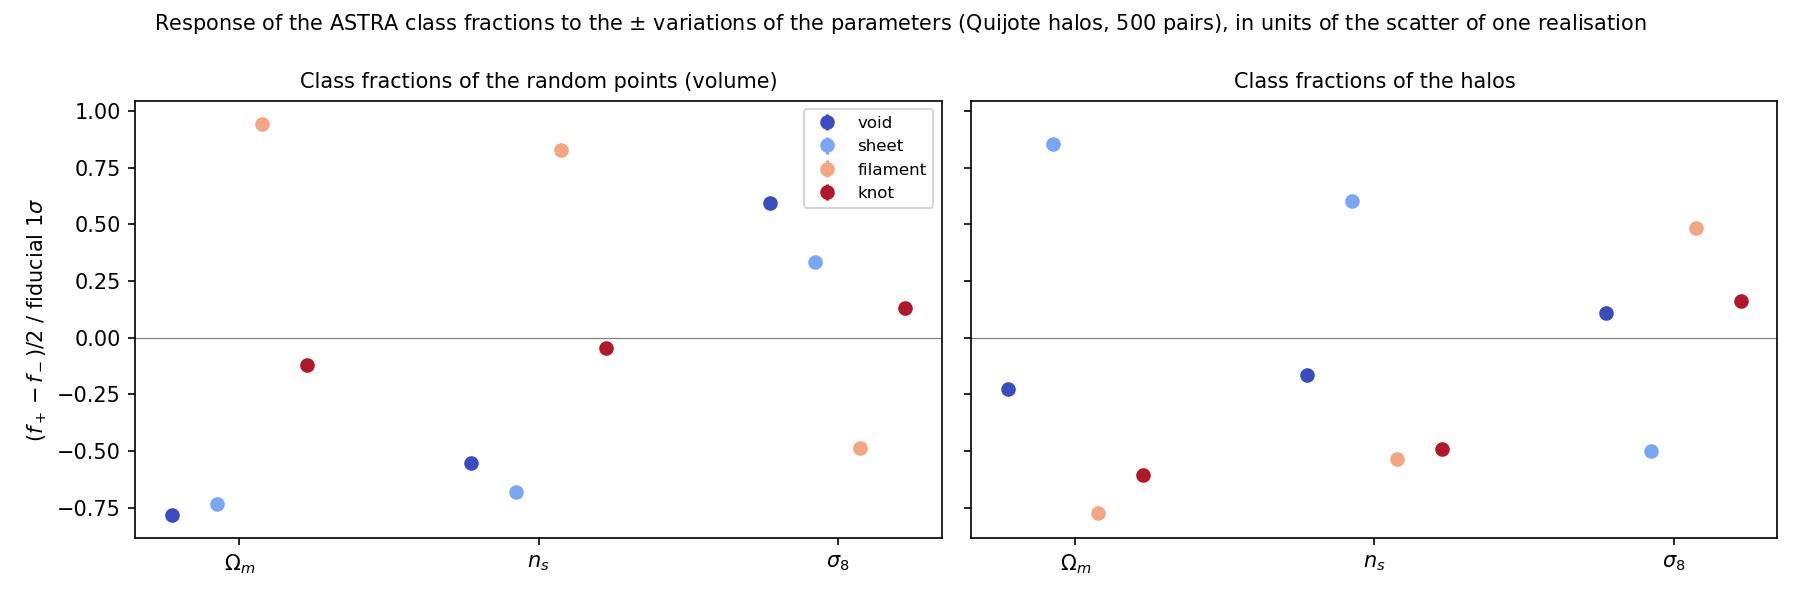
\includegraphics[width=\textwidth]{classes_response.png}
\caption{Response of the ASTRA class fractions of the random points (left) and halos (right) to the $\pm$ variations of $\Omega_m$, $n_s$ and $\sigma_8$ (Quijote, 500 pairs), in units of the scatter of one realisation (error bars: error of the mean, smaller than the symbols).}
\label{fig:classes_resp}
\end{figure*}

\begin{figure*}[!tp]
\centering
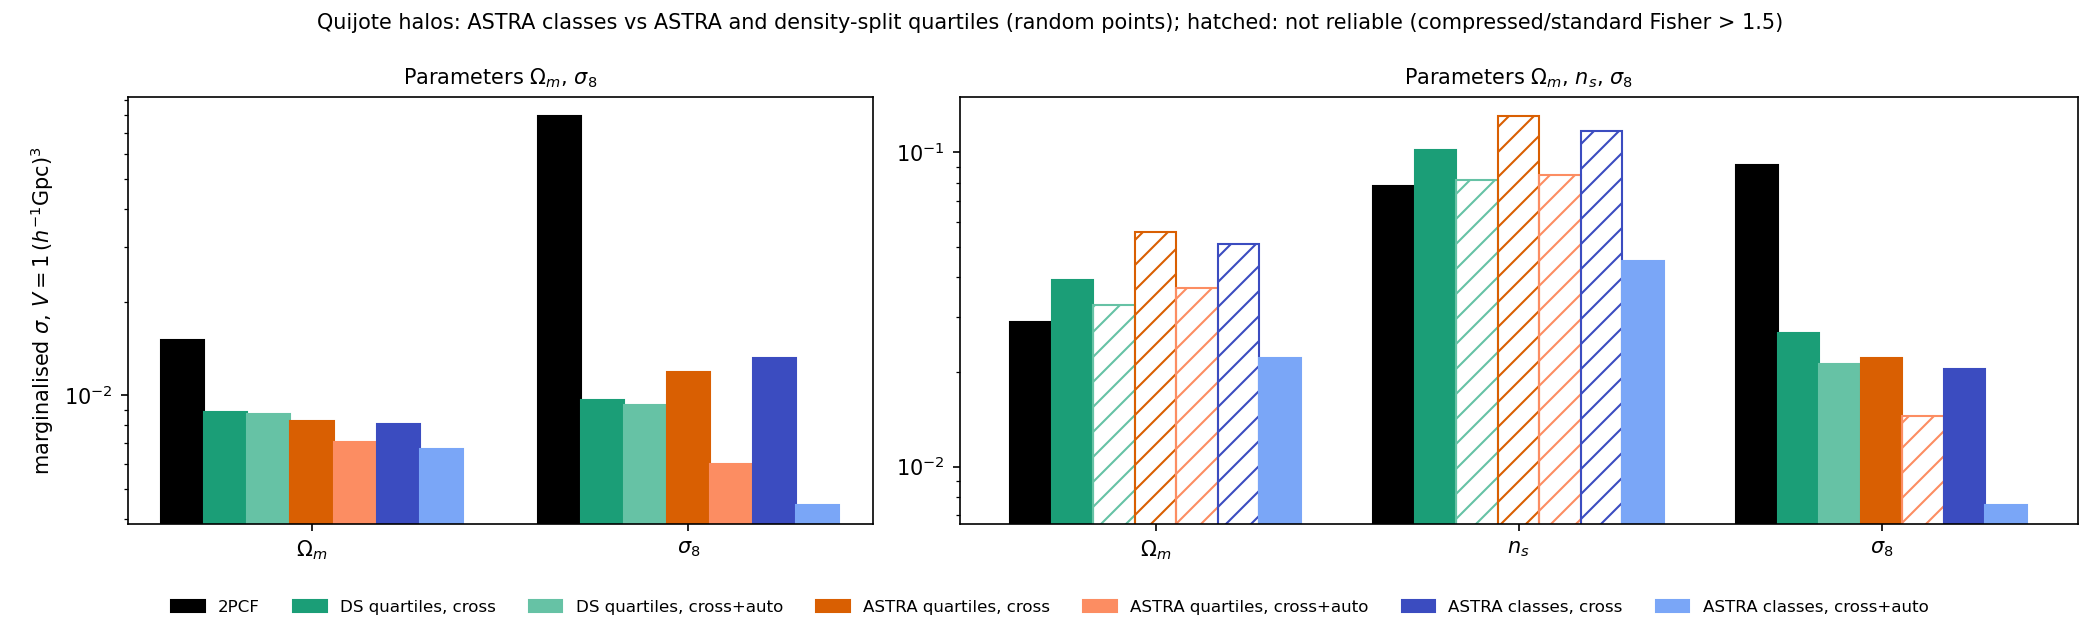
\includegraphics[width=\textwidth]{classes_fisher.png}
\caption{Quijote halos, $V=1\,(h^{-1}{\rm Gpc})^3$: marginalised errors for $(\Omega_m,\sigma_8)$ (left) and $(\Omega_m,n_s,\sigma_8)$ (right) from the 2PCF, the density-split and ASTRA quartiles of the random points, and the ASTRA classes (sheets and filaments), with cross-correlations only or with auto-correlations. Hatched: not reliable (compressed and standard Fisher estimators differ by more than a factor 1.5).}
\label{fig:classes_fisher}
\end{figure*}

\subsection{Inference with the emulator (MCMC)}
\label{sec:mcmc}

A Fisher forecast describes the likelihood by its curvature at the fiducial point: it assumes that the statistics vary linearly with the parameters around that point, so that the posterior is Gaussian, and it ignores the bounds of the prior. It can therefore miss non-Gaussian posteriors, degeneracies that bend, or parameters that hit their prior range. To test the full pipeline as it would be applied to data, we sampled the posterior of the 20 parameters (8 cosmological, 12 HOD) with the emulator as the model: Gaussian likelihood with the official covariance rescaled to the data volume plus the emulator error, uniform priors over the training range, \texttt{emcee} with 64 walkers and 8000 steps (Appendix~\ref{app:maths}). The data are measurements the emulator has never seen: one subvolume of each of 2 catalogues of the 8 test cosmologies, and 8 subvolumes of the official base box of the fiducial cosmology, each analysed with the 2PCF, ASTRA split, density split and their combinations (120 chains).

Nothing in the procedure forces the posteriors to be correct; whether they are is what this test measures. On average the posterior mean is offset from the truth by less than 0.4 posterior standard deviations for every parameter, and the truth lies within the $1\sigma$ interval in 69--100\% of the runs on held-out cosmologies (68\% expected for calibrated posteriors). This is reassuring but not a strong test: the posteriors are barely narrower than the priors (Figures~\ref{fig:mcmc} and~\ref{fig:mcmc_off}), their widths being 84--101\% of the prior widths, and a posterior close to the prior contains the truth by construction. One $(500\Mpch)^3$ volume with 12 free HOD parameters constrains $\omega_{\rm cdm}$ by 8--16\% beyond its prior, and the other parameters by less than 10\%, and the statistics differ by a few per cent. A first set of runs on the full $(2\,h^{-1}{\rm Gpc})^3$ box was limited the other way: there the emulator error is as large as the statistical error (Section~\ref{sec:emulator}) and masked the differences between the statistics. Distinguishing the statistics through inference requires both a large volume and an emulator error well below the statistical error of that volume, which the present training set cannot reach; the comparison of the methods rests on the Fisher forecasts, and the inference pipeline is validated and ready for a less noisy training set.

\begin{figure}[!htbp]
\centering
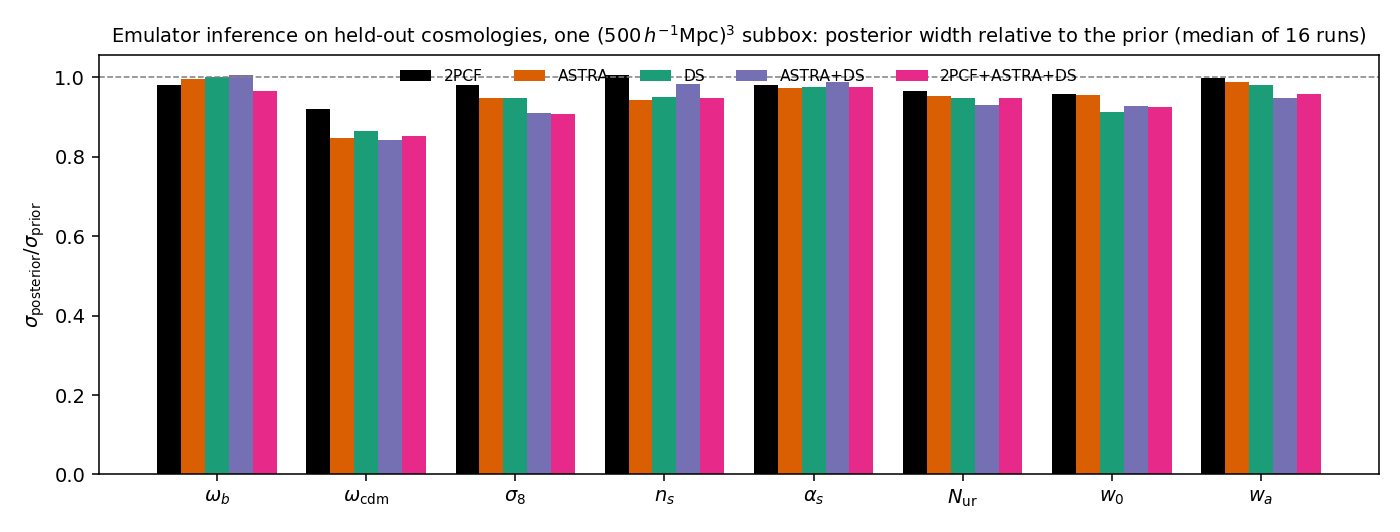
\includegraphics[width=\linewidth]{v2_mcmc_widths.png}
\caption{Emulator inference on held-out cosmologies (one $(500\Mpch)^3$ volume, official covariance): posterior width relative to the prior width, median of 16 runs, for the 2PCF, ASTRA split, density split and their combinations.}
\label{fig:mcmc}
\end{figure}

\begin{figure*}[!tp]
\centering
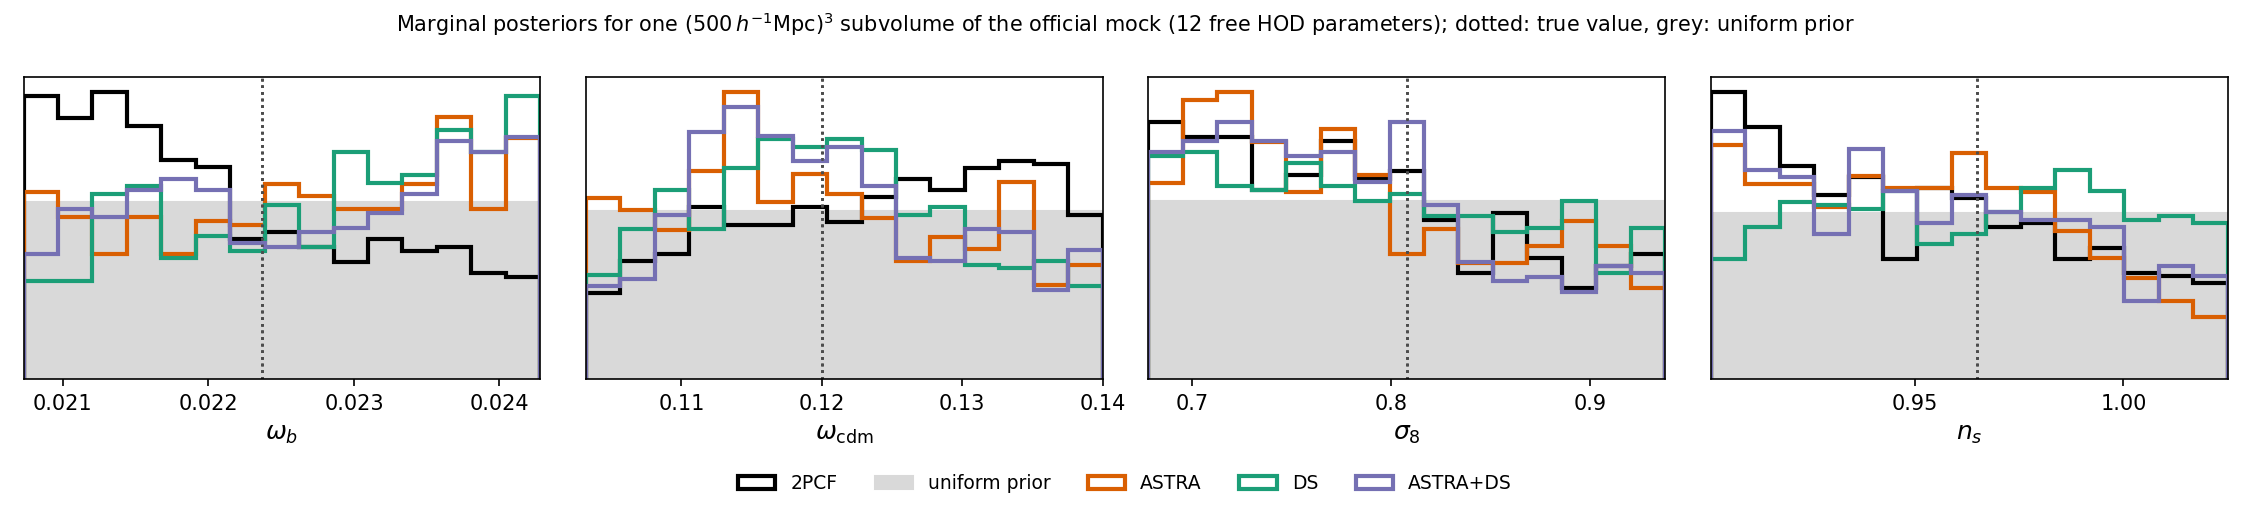
\includegraphics[width=\textwidth]{readable_mcmc_official.png}
\caption{Marginal posteriors of four cosmological parameters for one $(500\Mpch)^3$ subvolume of the official mock (fiducial cosmology, dotted lines), with 12 free HOD parameters, for the 2PCF, ASTRA split, density split and ASTRA + DS. At this volume all posteriors remain close to the uniform prior (grey).}
\label{fig:mcmc_off}
\end{figure*}


